\subsection{Time-Shift Regularization}
\label{appendix:regularization}


Beyond the architectural and task-based approaches, we experimented with regularization techniques. During deployment, we observed a consistent sensitivity to intent changes, suggesting the learned policies were overfitting to the expert policy in the training data. To address this, we implemented time-shift regularization, which involves shifting intent and velocity labels by a small number of time steps relative to the ground truth. This approach assumes that the expert policy is stochastic; therefore, intents or velocities remain valid across a range of time steps. We also hypothesized that this would increase robustness to latency errors, which accumulate when the model is deployed on a remote machine rather than locally on the Duckiebot.

To test this, we trained the FiLM architecture with various time-shift values and qualitatively evaluated its performance on the Duckiebot. The regularization was implemented as a Gaussian distribution around the ground truth timestamp (illustrated in Figure \ref{fig:time_shift_distributions}). Given the 10Hz data collection rate, we tested velocity and intent label shifts at a standard deviation of 0.1s, both independently and in combination. Additionally, we tested a combined shift using a standard deviation of 0.05s, both with and without a 0.05s mean shift into the future.

\begin{figure}[H]
    \centering
    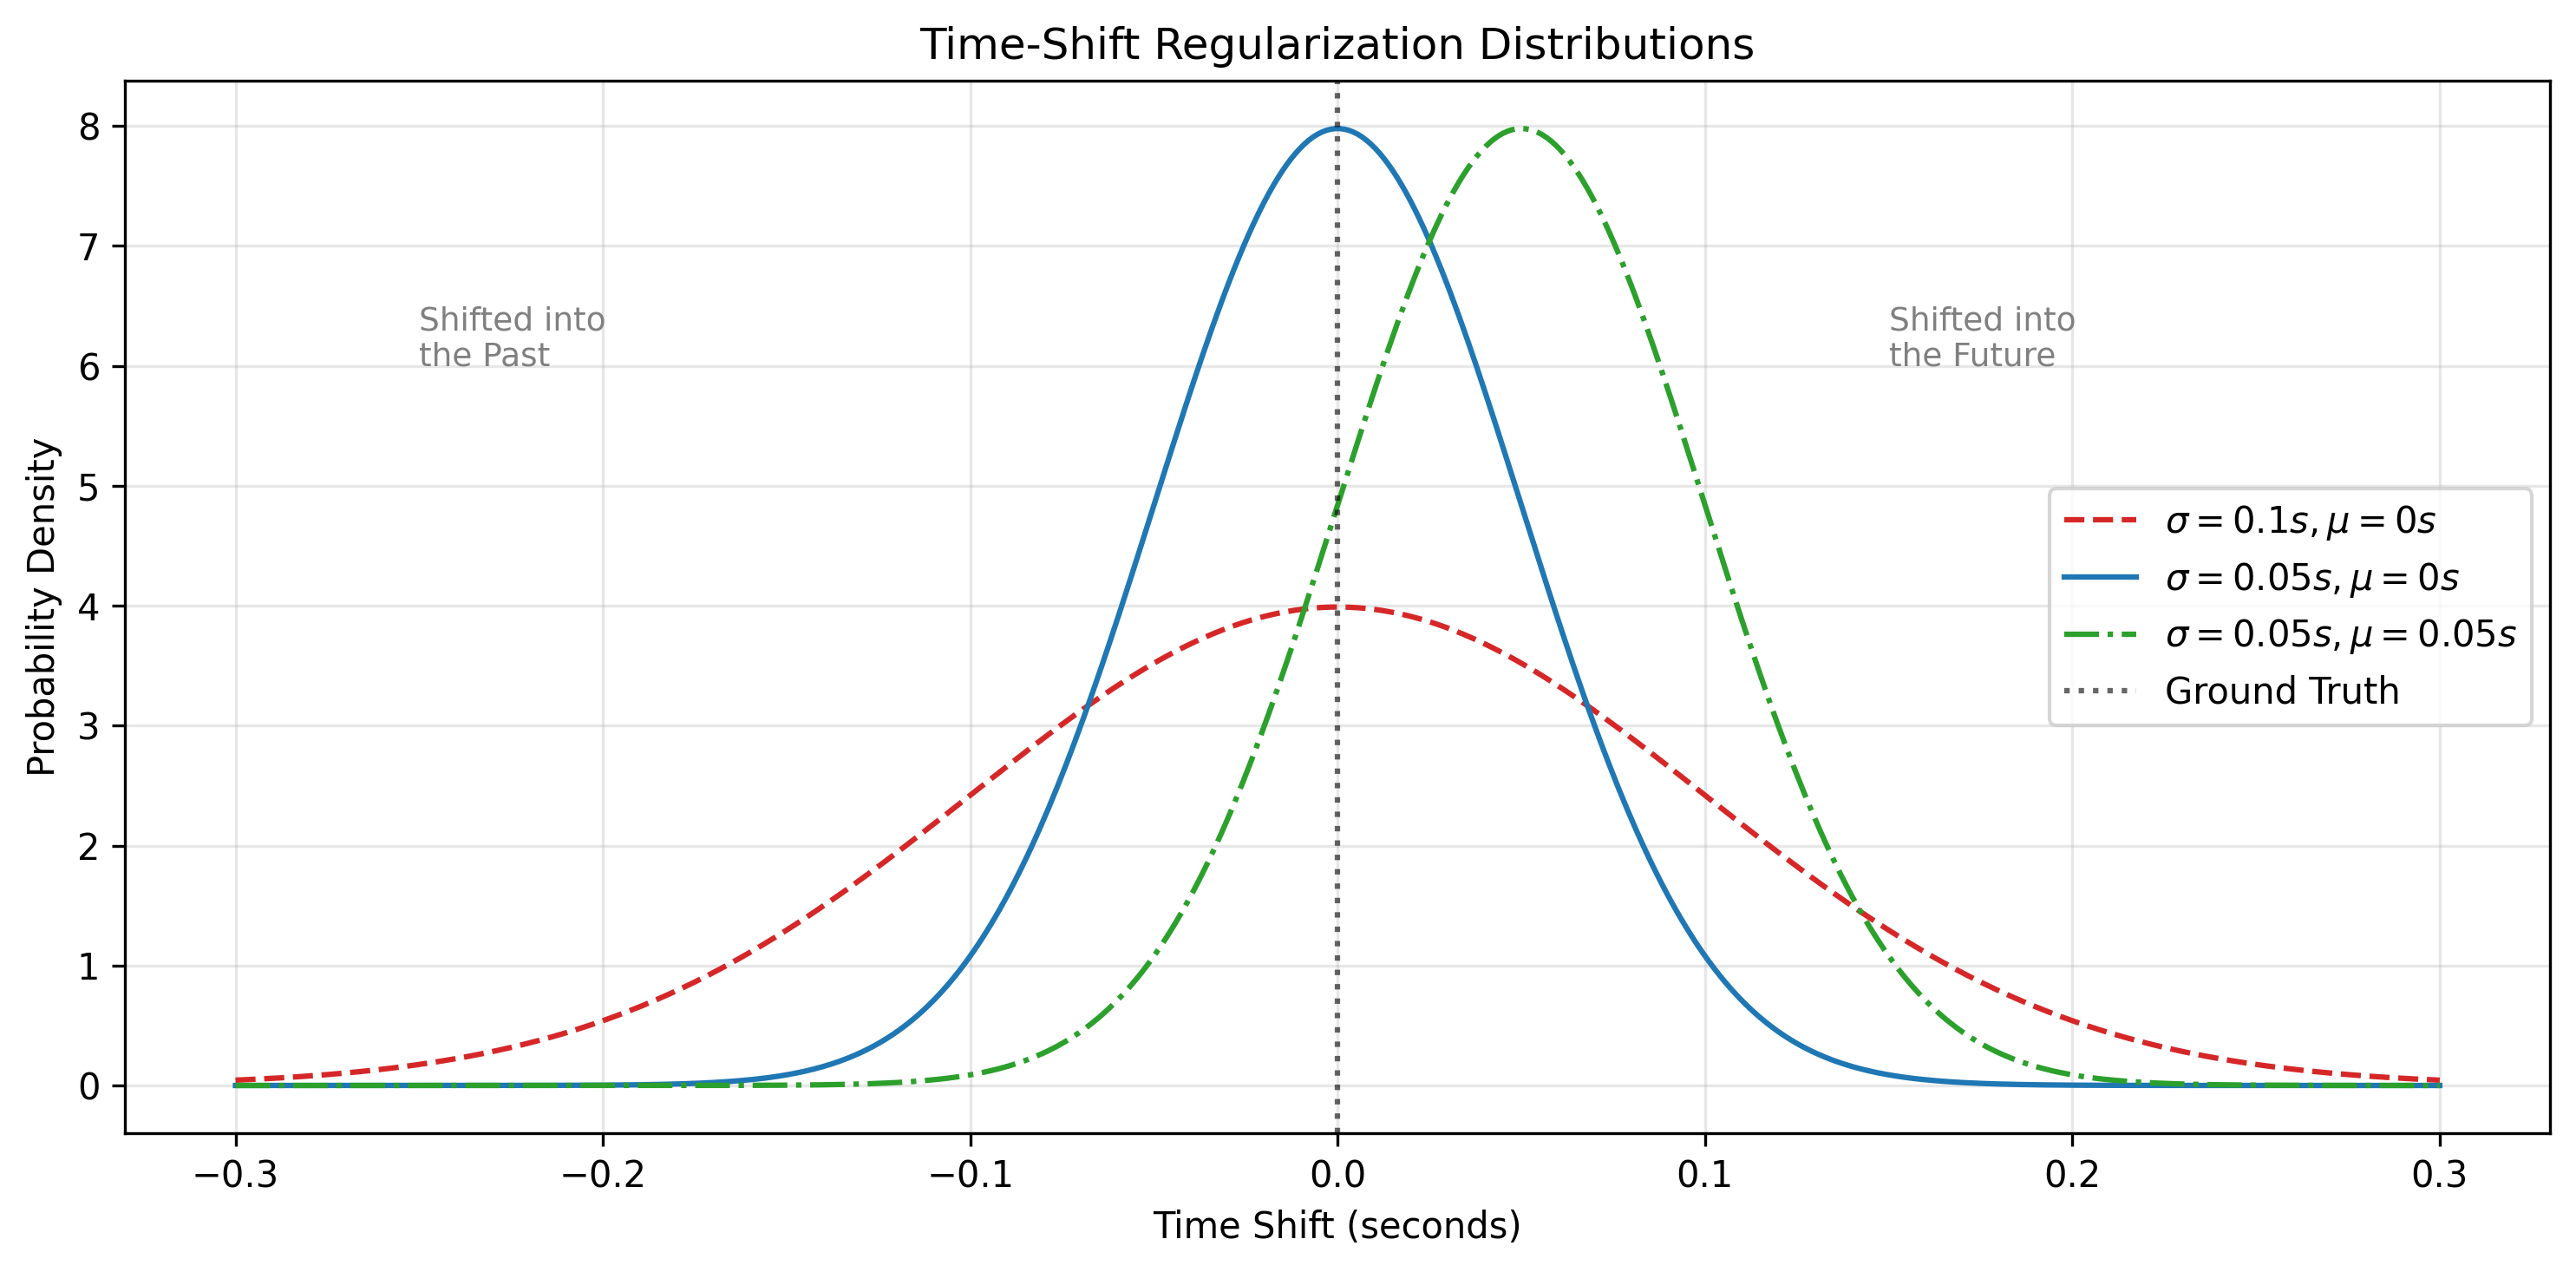
\includegraphics[width=0.8\textwidth]{images/ablation/regularization/time_shift_distributions.png}
    \caption{\textbf{Time-shift regularization:} The figure illustrates the Gaussian distributions used for time-shift regularization.}
    \label{fig:time_shift_distributions}
\end{figure}

Results indicated that these models generally underperformed compared to the baseline. Specifically, the Duckiebot frequently failed to maintain its lane and showed no significant improvement in intersection maneuvers. While the models improved at maintaining a straight path at intersections, they still trailed the baseline model trained with the sampling strategy described in Section \ref{sec:results}. Among the variants, the model with a 0.05s standard deviation and mean shift performed best, whereas all models with a 0.1s standard deviation performed worst. We suspect that shifting labels into the past causes the model to learn a policy that lacks the reactivity required for lane following. Shifting the Gaussian mean into the future reduced the likelihood of past-label shifts, likely accounting for that model’s superior performance. Given these results, we chose to prioritize other approaches rather than further investigate these temporal shifts.